\subsection{Unittesten}
Voor het unit testen van de API is er gebruikgemaakt van xUnit (voor meer informatie zie sectie \ref{section:Bouwomgeving}).
Unit testen worden gebruikt om de verschillende logica van het systeem te testen.
Hierom zijn testen geschreven voor de handlers en de data mappers in de applicatie.
Een voorbeeld van zo'n unit test is te zien in figuur \ref{fig:ExampleUnitTest}.
Verder is er een overzicht van de verschillende unittesten in figuur \ref{fig:OverviewUnitTests}.

\whitespace[2]
\begin{graphic}
	\captionsetup{type=figure}
	\caption{Geïmplementeerde unit test}
	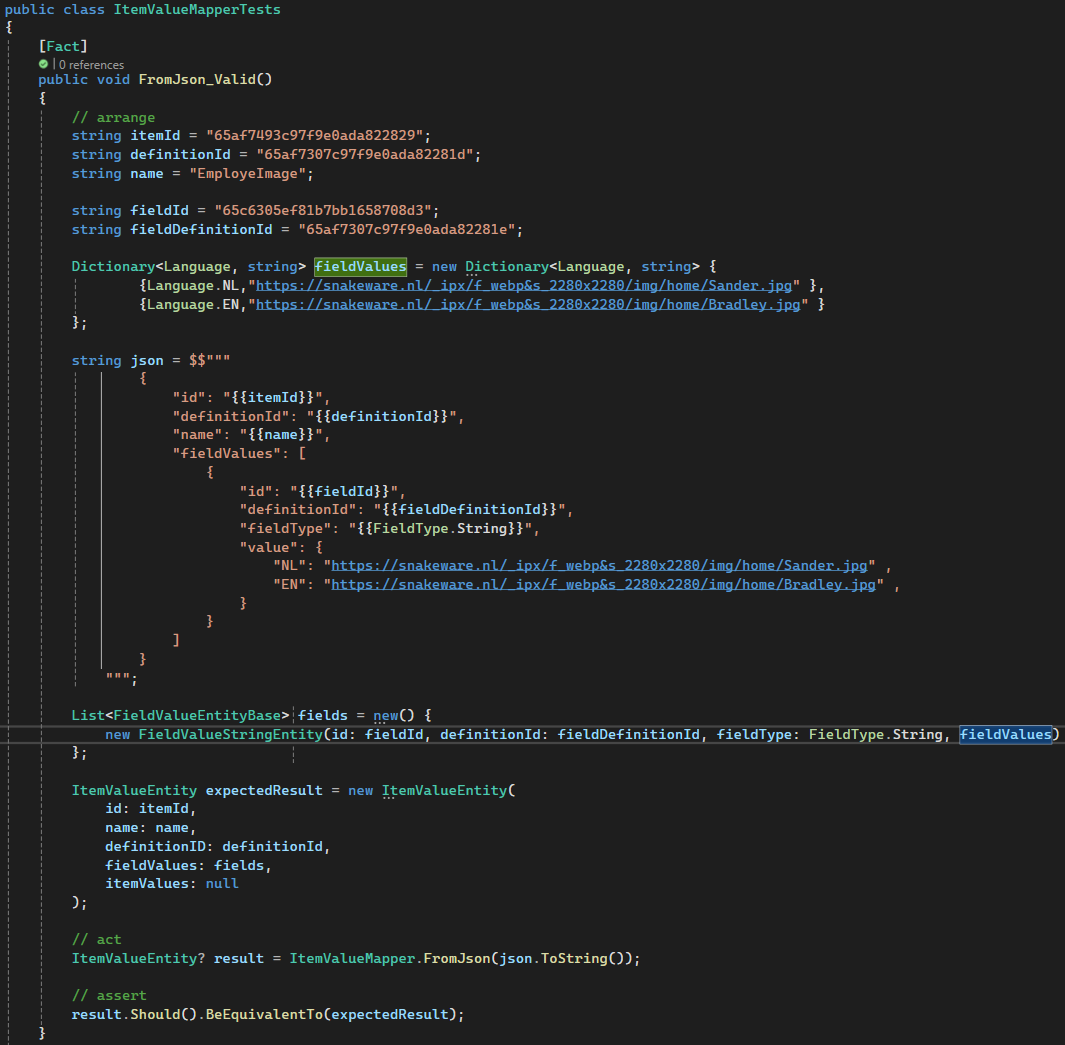
\includegraphics[scale=0.52]{ExampleUnitTest.png}
	\label{fig:ExampleUnitTest}
\end{graphic}
